\section{Miljön}
I det här avsnittet kommer vi att se exempel på hur vi kan använda Ansible för att konfigurera en uppsättning maskiner som ser ut ungefär som den uppsättning vi har i TDDI41. Vi börjar med att titta på strukturen över de fyra maskinerna, inte minst för de som inte är bekanta med kursens innehåll.

\begin{figure}[H]
  \center
  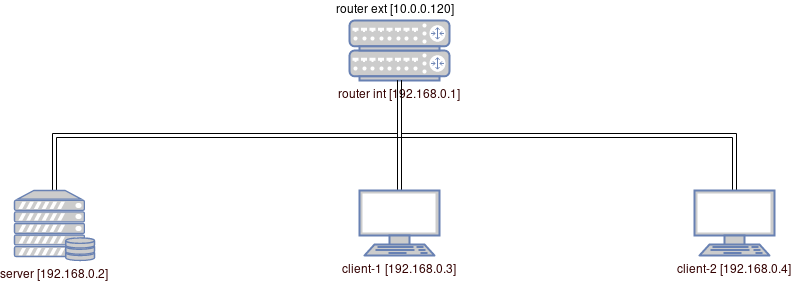
\includegraphics[scale=0.55]{./bilder/tddi41-overview.png}
  \caption{Överblick av noderna i TDDI41}
\end{figure}

Bilden är inte helt rättvisande då den refererar till interna ip-adresser (nätmask /24), 
men det är något vi inte bryr oss nämnvärt vid i det här fallet. Våra exempel kommer även
att förenkla det hela än mer och endast se till det inre nätet. Ett alternativt sätt att
se på det hela är att vi skulle använda enheten \texttt{router} som den maskin vi pushar
våra konfigurationer på. Anledningen till denna förenkling är för att fokusera på och 
tydliggöra själva Ansible-delen snarare än att lösa hela labbserien.
Vi kommer även förutsätta att vi har satt IP-adresser på maskinerna innan vi börjar med Ansible.

Enheten \texttt{router} är en maskin med dubbla nätverkskort (vi bortser från detta här som sagt) som,
precis som namnet antyder, agerar gateway till det inre nätverket samt ntp-server.
Enheten \texttt{server} är en maskin som agerar fillagring, autentiseringsserver, eventuell mailserver, med mera.
Enheterna \texttt{client-\emph{n}} är i det här avseendet identiska sånär som på namn och ip och
är huvudsakligen till för att skala upp miljön.

\section{Hur vi använder Ansible}
När vi vill pusha ändringar till våra noder kan vi använda två olika kommandon: \texttt{ansible} samt \texttt{ansible-playbook}.

Kommandot \texttt{ansible} är det råa kommandot där vi måste specifiera vilka moduler etc. vi skall använda, vilket kan användas för att exempelvis kolla att våra noder är uppe eller för att se variabler som samlas in från en nod. Vi återkommer till detta.

Kommandot \texttt{ansible-playbook} är det vi huvudsakligen kommer att använda oss utav när vi faktiskt pushar ändringar. Det kör då en specifik playbook som anger på vilka noder vad ska köras. Som vi kommer se kan vi göra många justeringar på många system samtidigt med hjälp av dessa playbooks.

\subsection{Vad händer vid en körning}
Om vi ser till vad som händer när vi kör en playbook så händer enkelt sett följande:
Vi ansluter via SSH till noden, skickar över de moduler tillsammans med variabler för hur dessa ska köras samt när, kör en modul som inhämtar körinformation i form av variabler från noden för att (eventuellt) använda dessa variabler tillsammans med de vi skickat med. Till sist kör vi då det script vi skickat över som använder överskickade moduler för att göra förändringarna på noden, och så skickar vi tillbaka körinformation till styrenheten som skriver ut hur det gick på skärmen.

Komplicerat? Ja, bakom ridån, men inte användningsmässigt. Låt oss titta vidare.

\section{Ett faktiskt exempel}
Vi kommer senare att gå in på hostfilen, syntaxer och så vidare, men låt oss först ta ett exempel där vi visar hur enkelt ett kommando för att konfigurera alla client-noder:

\texttt{\$ ansible-playbook clients.yml}

Skulle vi dessutom vilja ansluta som en särskild användare (\texttt{ansacc}), begränsa oss till en enda klient, begränsa de tasks vi 
vill köra till att endast inkludera NTP-konfiguration och dessutom bara testköra (inga förändringar på den faktiska 
noden), då skulle det kunna se ut som följande:

\texttt{\$ ansible-playbook clients.yml -u ansacc -k --limit client-1 --tags NTP -C}

Körkommandot kan i stort sett sköta det mesta, men vanligtvis vill vi ställa in så mycket som möjligt i konfigurationsfilerna, dels Ansibles, men även hostspecifika och gruppspecifika, men mer om det under \ref{sec:bestpractices} Best practices.
